% =====================================================================
%  §4. Линейная аппроксимация: гармоники закона Малюса
%
%  ЖАНР (STYLE.md): учебная литература. Ни путей, ни имён программ, ни
%  номеров гипотез. Прослеживаемость — ключи \srckey{4.x} и приложение.
%
%  Содержательная основа: research/two_wgp/NOTE_malus_linearization.md
%  (обучающий разбор с выводом; markdown первичен по фактуре).
% =====================================================================
\section{Линейная аппроксимация: гармоники закона Малюса}
\label{sec:linear-fit}
\markboth{§\thesection. Линейная аппроксимация}{}

Части~II этого курса предстоит подгонять модель к измеренной угловой развёртке~--- в общем случае
нелинейную задачу с итерациями, стартовыми точками и риском застрять не в том решении
(аппарат для этого появится в §7). Но прежде чем разбираться с этими трудностями, стоит заметить:
часть той же самой информации~--- офсет угла, амплитуды каналов, их относительная
фаза~--- извлекается \emph{без единой итерации}, обычным линейным методом наименьших квадратов, с
единственным глобальным минимумом и точной, а не приближённой, оценкой ошибки. Это не хитрость и
не частный случай~--- это следствие одного тригонометрического тождества, применённого к
выражению~\eqref{eq:two-channels}, которое курс вывел ещё в §0.

\begin{tcolorbox}[enhanced,colback=cPanel,colframe=cGrid,boxrule=0.8pt,arc=2pt,
                  title={\bfseries\color{cAccent} Пререквизиты},coltitle=cAccent,
                  attach boxed title to top left={xshift=6pt,yshift=-2pt},
                  boxed title style={colback=cPanel,boxrule=0pt,arc=0pt},top=10pt]
\textbf{Нужно знать:} формулы~\eqref{eq:two-channels}--\eqref{eq:U-cross} из §0 (поле~$\Efield(\theta)$
и энергия~$U(\theta)$ с перекрёстным членом); тригонометрическая формула понижения степени
$\cos^2\alpha=\tfrac12(1+\cos2\alpha)$; метод наименьших квадратов как решение нормального
уравнения линейной регрессии.\\[0.3em]
\textbf{Знать НЕ нужно:} нелинейную оптимизацию, алгоритм Левенберга--Марквардта~--- в этом
параграфе он не нужен вовсе, и это главная мысль параграфа.
\end{tcolorbox}

% ---------------------------------------------------------------------
\subsection{Идея: неудобная нелинейность на самом деле не нелинейность}
\label{subsec:idea}

\begin{intuition}
Классический закон Малюса записывают как «яркость~--- квадрат косинуса угла». Квадрат косинуса
выглядит неудобно: сам по себе он нелинеен по углу~$\theta$, а офсет~$\theta_0$~--- неизвестный
ноль шкалы прибора~--- сидит \emph{внутри} косинуса, что обычно требует итерационной подгонки.
Но школьное тождество $\cos^2\alpha=\tfrac12(1+\cos2\alpha)$ говорит: квадрат косинуса~--- это не
нелинейность, а косинус \emph{удвоенного} угла плюс константа. Модуляция происходит на удвоенной
частоте вращения~--- поворот на $180^\circ$ возвращает картину в исходное состояние, потому что
поляризатор не различает <<вперёд>> и <<назад>>.
\end{intuition}

Возьмём учебную (интенсивностную) форму закона Малюса, $U(\theta)=U_{\min}+(U_{\max}-U_{\min})
\cos^2(\theta-\theta_0)$, и применим тождество:
\begin{equation}
  U(\theta)=a_0+a_1\cos2\theta+b_1\sin2\theta,
  \label{eq:linear3}
\end{equation}
где $a_0=\tfrac12(U_{\max}+U_{\min})$, а $a_1,b_1$~--- некоторая пара чисел, зависящая от
$U_{\max}-U_{\min}$ и~$\theta_0$ (явные формулы~--- в §\ref{subsec:closed-form}).

\begin{strict}[: что произошло с офсетом]
Неизвестный угол~$\theta_0$ был аргументом косинуса~--- нелинейным параметром. После разложения он
«вышел наружу» и распределился между двумя \emph{линейными} коэффициентами $a_1,b_1$. Базисные
функции $1,\cos2\theta,\sin2\theta$ от неизвестных параметров не зависят~--- это фиксированный,
заранее известный набор функций угла. Значит, \eqref{eq:linear3}~--- обычная линейная регрессия, а
не итерационная задача.
\end{strict}

\begin{intuition}[: это стандартный приём метрологии]
Тот же самый ход~--- искать неизвестный офсет не подгонкой аргумента, а разложением по гармоникам
удвоенного угла~--- давно применяется в оптической метрологии вращающегося элемента (эллипсометрия
с вращающимся анализатором, синхронное детектирование на второй гармонике). Курс применяет его не
ко времени, а к угловой развёртке~--- идея та же.
\end{intuition}

% ---------------------------------------------------------------------
\subsection{Почему нужна четвёртая гармоника}
\label{subsec:fourth-harmonic}

Форма~\eqref{eq:linear3}~--- учебная: она верна для \emph{некогерентной} (интенсивностной)
композиции каналов. Но §0 установил (формула~\eqref{eq:two-channels}), что наша установка
складывает \emph{поля}, а не мощности, и лишь потом берёт квадрат модуля. Применим то же
тождество понижения степени прямо к полю:
\begin{equation}
  \Efield(\theta)=\tperp\cos^2\theta+\tpar\sin^2\theta
  = A+B\cos2\theta,
  \qquad
  A=\tfrac12(\tperp+\tpar),\quad B=\tfrac12(\tperp-\tpar).
  \label{eq:field-linear}
\end{equation}
Поле линейно по $\cos2\theta$~--- многочлен первой степени. Но наблюдаемая~--- это
$U=|\Efield|^2$, а квадрат многочлена первой степени по $\cos2\theta$ содержит $\cos^22\theta$,
которое тем же тождеством понижения степени даёт $\cos4\theta$. Итого \textbf{точно}, без всякого
приближения:
\begin{equation}
  U(\theta)=c_0+a_2\cos2\theta+b_2\sin2\theta+a_4\cos4\theta+b_4\sin4\theta .
  \label{eq:linear5}
\end{equation}

\begin{warning}[: это тождество, а не аппроксимация]
Разложение~\eqref{eq:linear5} не отбрасывает никаких членов и не является рядом, обрезанным на
каком-то порядке. Квадрат модуля линейной по $\cos2\theta$ величины~--- \emph{ровно}
тригонометрический многочлен 4-й степени, и точнее пяти коэффициентов~\eqref{eq:linear5} для его
описания не требуется. Это ровно то же тождество, что дало формулу~\eqref{eq:U-cross} в §0, только
здесь оно доведено до готового линейного базиса.
\end{warning}

\begin{example}[: точность тождества на практике]\srckey{4.1}
Прямая численная проверка формы~\eqref{eq:linear5} против полного выражения~\eqref{eq:U-cross} на
измеренных частотных сетках даёт относительное среднеквадратичное расхождение порядка
$10^{-16}$~--- машинный ноль (тот же результат, что уже приводился в §0 как ключ~0.2, здесь~---
подтверждение того, что он справедлив построчно, на уровне отдельной частоты, а не только в
среднем).
\end{example}

\begin{tcolorbox}[enhanced,colback=cS1!7,colframe=cS1,boxrule=0pt,leftrule=3pt,arc=1pt]
\textbf{Учебная 3-параметрическая форма~\eqref{eq:linear3} для нашей установки систематически
неполна}: она отбрасывает четвёртую гармонику, которая, как было установлено в §0, несёт около
четверти всего сигнала~--- и, что важнее, несёт единственную информацию об относительной фазе
каналов (следующий пункт).
\end{tcolorbox}

% ---------------------------------------------------------------------
\subsection{Замкнутые формулы: от коэффициентов обратно к физике}
\label{subsec:closed-form}

Три коэффициента $c_0,c_2,c_4$ (где $c_2=\sqrt{a_2^2+b_2^2}$, $c_4$~--- аналогично для четвёртой
гармоники, с точностью до знака, обсуждаемой ниже) связаны с тремя физическими величинами
взаимно однозначно:
\begin{equation}
  |\tperp|^2=c_0+c_2+c_4,
  \qquad
  |\tpar|^2=c_0-c_2+c_4,
  \qquad
  \Real(\tperp\overline{\tpar})=c_0-3c_4 .
  \label{eq:closed-form}
\end{equation}
Отсюда~--- \term{модельно-независимо}, одним решением линейной системы, без какого-либо
предположения о механизме, породившем $\tperp,\tpar$:
\[
  \eta=\left|\frac{\tpar}{\tperp}\right|
  =\sqrt{\frac{c_0-c_2+c_4}{c_0+c_2+c_4}},
  \qquad
  \cos\Delta\varphi=\frac{c_0-3c_4}{\sqrt{(c_0+c_2+c_4)(c_0-c_2+c_4)}} .
\]

\begin{intuition}[: самый красивый момент этого параграфа]
Относительная фаза каналов $\Delta\varphi$~--- физическая величина, за которой мы гонялись ещё с
§0 ($\tleak$~--- это её наклон по частоте,~--- и с §1, где просачивание получило и амплитуду,
и фазу,~--- входит в формулы \eqref{eq:closed-form} \textbf{только через}~$c_4$. В интенсивностной
трёхпараметрической картине фазы нет вообще~--- она там принципиально ненаблюдаема. Учебная
линеаризация~\eqref{eq:linear3} слепа к $\Delta\varphi$ не приблизительно, а точно: она
выбрасывает ровно ту гармонику, которая единственная её несёт.
\end{intuition}

\begin{strict}[: два бесплатных теста корректности]
Формулы~\eqref{eq:closed-form} дают два внутренних теста, которых нет в нелинейной подгонке:
\begin{enumerate}[leftmargin=1.6em,itemsep=0.2em]
  \item \term{Неравенство Коши--Буняковского} $|\Real(\tperp\overline{\tpar})|\le|\tperp||\tpar|$,
        то есть $|\cos\Delta\varphi|\le1$. Нарушение означает, что данные не описываются схемой
        «один вращающийся элемент, дающий поле по формуле~\eqref{eq:field-linear}»~--- сигнал
        каких-либо помех к сигналу.
  \item \term{Согласие двух независимых оценок офсета}: $\theta_0=\tfrac12\operatorname{atan2}(b_2,a_2)$
        из второй гармоники и $\theta_0=\tfrac14\operatorname{atan2}(b_4,a_4)\pmod{45^\circ}$ из
        четвёртой обязаны совпасть, если данные действительно порождены одним и тем же
        вращающимся элементом.
\end{enumerate}
\end{strict}

% ---------------------------------------------------------------------
\begin{figure}[t]
  \centering
  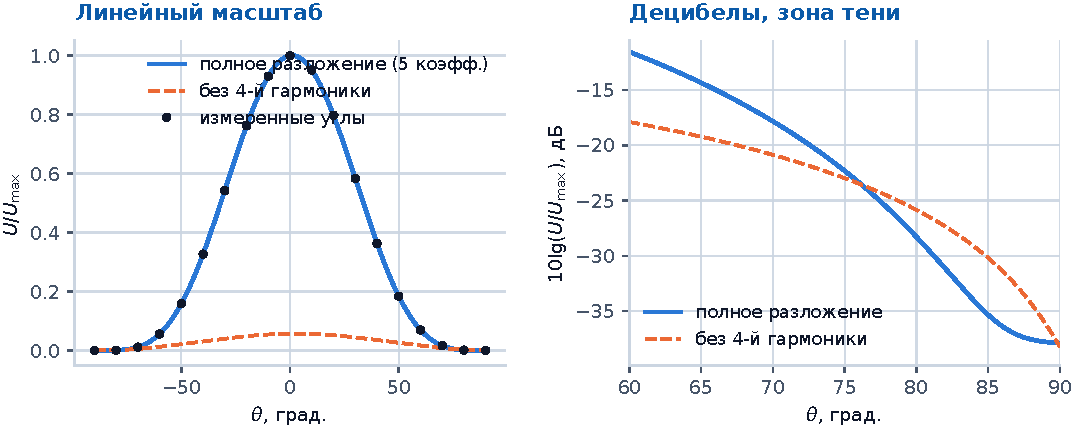
\includegraphics[width=\linewidth]{figures/fig04_harmonics_decomp.pdf}
  \caption{Плотная решётка ($D/P=0{,}71$, ключ~4.2): измеренная угловая развёртка (энергия,
  просуммированная по рабочей полосе частот) и её восстановление по формуле~\eqref{eq:linear5} со
  всеми пятью коэффициентами против восстановления без четвёртой гармоники. В районе максимумов
  разница не видна; вблизи $90^\circ$, где сосредоточено просачивание, отбрасывание четвёртой
  гармоники даёт заметный систематический сдвиг~--- та же четверть сигнала, о которой шла речь
  выше, теряется именно там, где она важнее всего.}
  \label{fig:harmonics-decomp}
\end{figure}

% ---------------------------------------------------------------------
\subsection{Аппарат линейного МНК}
\label{subsec:lsq}

Запишем~\eqref{eq:linear5} как задачу линейной регрессии. Пусть измерено $N$ значений $U_i$ на
углах~$\theta_i$. \term{Матрица плана}~$X$ имеет $N$ строк и пять столбцов:
\[
  X=\big[\,1,\ \cos2\theta_i,\ \sin2\theta_i,\ \cos4\theta_i,\ \sin4\theta_i\,\big]_{i=1\ldots N},
\]
и решение~--- обычные нормальные уравнения взвешенного МНК:
\begin{equation}
  \mathbf{p}=(X^{\mathsf T}WX)^{-1}X^{\mathsf T}W\mathbf{y},
  \qquad
  \operatorname{Cov}(\mathbf{p})=(X^{\mathsf T}WX)^{-1},
  \qquad
  W=\operatorname{diag}(1/\sigma_i^2) .
  \label{eq:normal-eq}
\end{equation}
Ни итераций, ни стартовой точки, ни риска сойтись не туда: система линейна, решение~--- одно
решение линейной алгебры, ковариация~--- точная (не приближение вблизи минимума, как это будет
в §7--§9 для нелинейной задачи).

\begin{intuition}[: откуда берётся ковариация без всякой статистики Монте-Карло]
Для линейной регрессии с гауссовым шумом оценка коэффициентов~$\mathbf{p}$~--- сама линейная
комбинация данных, и её ковариация выражается через ковариацию данных \emph{в замкнутом виде}
матричной формулой $(X^{\mathsf T}WX)^{-1}$. Бутстрап или другие ресемплинговые методы (§7) здесь
попросту не нужны~--- они нужны там, где такой формулы нет.
\end{intuition}

\paragraph{Дельта-метод.} Величины вроде $\theta_0$~--- нелинейные функции коэффициентов
$a_2,b_2$, и напрямую их ковариация из~\eqref{eq:normal-eq} не следует. Но раз ковариация
коэффициентов известна точно, ошибку любой гладкой функции от них~--- в частности,
$\theta_0=\tfrac12\operatorname{atan2}(b_2,a_2)$~--- даёт стандартный \term{дельта-метод}
(линеаризация функции первой производной):
\[
  \sigma^2(\theta_0)=\frac{b_2^2\operatorname{Var}(a_2)+a_2^2\operatorname{Var}(b_2)
  -2a_2b_2\operatorname{Cov}(a_2,b_2)}{4(a_2^2+b_2^2)^2} .
\]
В частном, но практически важном случае~--- углы равномерно покрывают полный период по
$2\theta$~--- матрица $X^{\mathsf T}X$ диагональна, и формула сворачивается до
$\sigma(\theta_0)=\sigma_U/(c_2\sqrt{2N})$: точность офсета определяется отношением шума к
амплитуде модуляции и числом точек~--- простая и полезная оценка при планировании измерения.

% ---------------------------------------------------------------------
\subsection{Урок про веса: шкала, в которой вы смотрите на данные, решает, что вы способны измерить}
\label{subsec:weights}

Матрица~$X$ не зависит от данных, но веса~$W$ выбираются, и выбор небезобиден.

\begin{warning}[: невзвешенный МНК заглушает тень]
Невзвешенный МНК по энергии эффективно взвешивает точку пропорционально~$U_i^2$ (обычная сумма
квадратов невязок весит большие значения тяжелее). Яркая зона (канал пропускания, малые углы)
на два--три порядка превосходит по величине тень (канал подавления, углы вблизи $90^\circ$)~---
и невзвешенный фит попросту не замечает тень, хотя именно там сосредоточена вся информация о
просачивании (§\ref{subsec:leakage}).
\end{warning}

\begin{example}[: до какой степени это ломает результат]\srckey{4.3}
На одном из образцов с относительно слабым просачиванием невзвешенная подгонка дала
$|\tpar|^2<0$~--- физически невозможный результат: оценка энергии отрицательна. Это не сбой
арифметики, а прямое следствие того, что тень, где $|\tpar|^2$ реально определяется, была
статистически невидима для невзвешенного МНК.
\end{example}

\noindent
Решение~--- веса $\sigma_i\propto U_i$ (постоянная \emph{относительная} ошибка, а не абсолютная).
Задача остаётся линейной: веса не зависят от искомых параметров, только от самих измерений,
поэтому формула~\eqref{eq:normal-eq} применяется без изменений.

\begin{example}[: два независимых теста сходятся до сотых долей градуса]\srckey{4.4}
При относительном взвешивании два независимых способа оценить офсет~--- из второй гармоники и из
четвёртой (тест из §\ref{subsec:closed-form}) сходятся с точностью
$0{,}004^\circ$--$0{,}05^\circ$ на всех образцах, для которых есть измерения. Совпадение,
полученное \emph{без единого предположения о верности физической модели}~--- просто как следствие
внутренней непротиворечивости данных,~--- сильный аргумент за то, что развёртка действительно
описывается одним вращающимся элементом.
\end{example}

\begin{center}
\footnotesize
\setlength{\tabcolsep}{6pt}
\begin{tabular}{@{}lrrrr@{}}
\toprule
\textbf{Образец} & \textbf{$\theta_0$, равном.} & \textbf{$\theta_0$, относит.} & \textbf{$\eta$,
равном.} & \textbf{$\eta$, относит.}\\
\midrule
плотная решётка, $D/P=0{,}71$        & $-0{,}097^\circ$ & $+0{,}901^\circ\pm0{,}184$ & $0{,}0347$ & $0{,}0127$ \\
повторная установка, $D/P=0{,}69$ (а) & $-0{,}286^\circ$ & $-0{,}546^\circ\pm0{,}248$ & \emph{отриц.} & $0{,}0121$ \\
повторная установка, $D/P=0{,}69$ (б) & $-0{,}654^\circ$ & $-0{,}463^\circ\pm0{,}198$ & $0{,}0478$ & $0{,}0130$ \\
разреженный образец, $D/P=0{,}46$    & $+0{,}211^\circ$ & $+0{,}599^\circ\pm0{,}327$ & $0{,}0373$ & $0{,}0329$ \\
\bottomrule
\end{tabular}
\end{center}
\srckey{4.5}
\noindent\emph{«Равномерные» веса~--- $\sigma_i=\mathrm{const}$; «относительные»~---
$\sigma_i\propto U_i$. Ошибка $\theta_0$~--- дельта-метод, поправленный на неизвестный масштаб
шума данных (поправка Бирджа); бутстрап не требуется. У образца (а) равномерные веса дают
физически невозможную (отрицательную) оценку энергии тени, поэтому столбец $\eta$ для него пуст.}

% ---------------------------------------------------------------------
\begin{figure}[t]
  \centering
  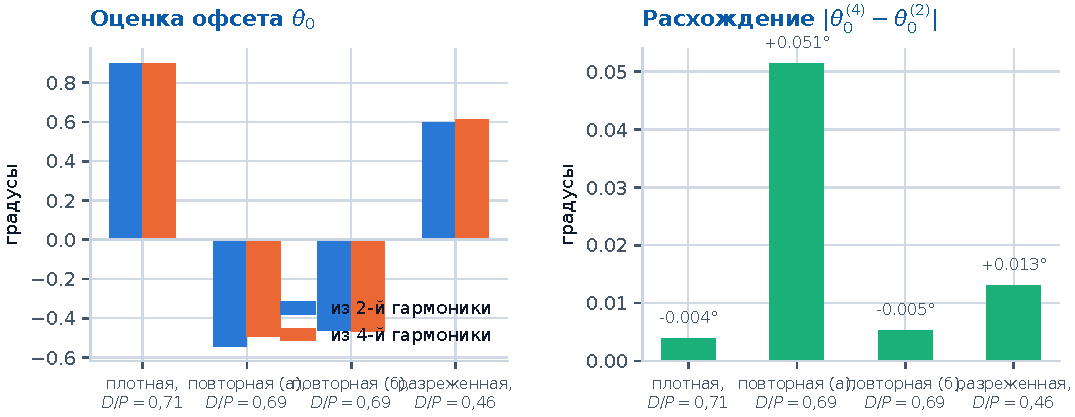
\includegraphics[width=\linewidth]{figures/fig04_weights.pdf}
  \caption{Согласие двух независимых оценок офсета~--- из второй и из четвёртой гармоники
  (§\ref{subsec:closed-form})~--- при относительном взвешивании $\sigma_i\propto U_i$: разница
  на всех образцах не превышает сотых долей градуса. Это внутренний тест непротиворечивости,
  а не сравнение с какой-либо независимо известной величиной.}
  \label{fig:weights}
\end{figure}

\begin{tcolorbox}[enhanced,colback=cS1!7,colframe=cS1,boxrule=0pt,leftrule=3pt,arc=1pt]
\textbf{Правило, впервые сформулированное в §1 (ключ~1.1) и подтверждённое здесь числом.} Шкала,
в которой вы взвешиваете данные, определяет, какие параметры вы способны измерить. Здесь это не
абстрактный тезис, а конкретная развилка: одни и те же измерения дают то отрицательную (невозможную)
оценку энергии тени, то физически осмысленный результат, совпадающий с независимой проверкой до
сотых долей градуса,~--- в зависимости только от выбора весов.
\end{tcolorbox}

% ---------------------------------------------------------------------
\subsection{Что ломает линейность, а что — нет}
\label{subsec:limits-linear}

Список того, что \emph{не} нарушает разложение~\eqref{eq:linear5} (доказано аналитически или
проверено численно), полезен не меньше списка ограничений: он избавляет от лишней осторожности
там, где она не нужна.

\begin{center}
\footnotesize
\setlength{\tabcolsep}{6pt}
\begin{tabular}{@{}p{0.34\linewidth}p{0.61\linewidth}@{}}
\toprule
\textbf{Не ломает} & \textbf{Почему} \\
\midrule
Частотная зависимость каналов & На каждой частоте своя пара $\tperp(\nu),\tpar(\nu)$~--- свои
$c_0,c_2,c_4$; структура~\eqref{eq:linear5} сохраняется частотно-поточечно \\
Фазовый член просачивания & Входит только в $\Real(\tperp\overline{\tpar})$, то есть только в
$c_4$; порядок многочлена не меняется \\
Суммирование по частотам & Сумма многочленов 4-й степени~--- снова многочлен 4-й степени \\
Второй (реальный) элемент тракта при выровненной оси & Теорема §\ref{subsec:alignment} даёт
общий скалярный множитель, не зависящий от $\theta$; отношения $\eta,\cos\Delta\varphi$ к нему
нечувствительны \\
\bottomrule
\end{tabular}
\end{center}

\begin{warning}[: а вот это ломает]
\textbf{Работа в децибелах.} Логарифм от тригонометрического многочлена~--- не многочлен: прямая
проверка даёт относительное расхождение порядка процента, когда та же процедура применяется к
$\lg U$ вместо~$U$. Разложение~\eqref{eq:linear5} нужно применять к самой энергии, а в
логарифмический масштаб переходить только для показа результата, не для его получения.
\textbf{Многолучевая интерференция} между элементами тракта тоже ломает структуру~--- она вносит
рациональную (а не полиномиальную) зависимость от $\cos2\theta$, то есть бесконечный ряд
гармоник; проверяется контролем гармоник шестого порядка и выше, которых в идентичности не
предусмотрено.
\end{warning}

% ---------------------------------------------------------------------
\subsection{Типичные ошибки этого параграфа}

\begin{enumerate}[leftmargin=1.6em,itemsep=0.25em]
  \item Использовать трёхпараметрическую (учебную) форму~\eqref{eq:linear3} для когерентной
        установки. Она отбрасывает четвёртую гармонику~--- четверть сигнала и всю фазу
        просачивания.
  \item Подгонять $\lg U$ или дБ вместо самой энергии~$U$. Логарифм многочлена~--- не многочлен;
        разложение перестаёт быть точным (§\ref{subsec:limits-linear}).
  \item Использовать одинаковые (не относительные) веса при большом динамическом диапазоне
        данных: яркая зона статистически заглушает тень, где сосредоточена вся интересующая
        физика (§\ref{subsec:weights}).
  \item Забыть проверить неравенство Коши--Буняковского для полученных $\tperp,\tpar$~--- это
        бесплатный тест, который нелинейная подгонка (§7) не предоставляет автоматически.
  \item Спутать согласие двух оценок офсета (внутренний тест непротиворечивости данных) с
        подтверждением физической модели: оно проверяет только то, что развёртку действительно
        произвёл один вращающийся элемент, а не то, какая модель верно описывает~$\tperp,\tpar$.
\end{enumerate}

\clearpage
